\chapter{Fejlesztést segítő eszközök}

Az alkalmazás készítése során igénybe vettem néhány olyan szolgáltatást, amelyek bár extra funkcionalitást nem adnak hozzá a kódbázishoz,
de nagyban megkönnyítik a fejlesztést végzők munkáját.

A Continuous Integration / Continuous Delivery egy manapság már általánosan használt módszer az alkalmazások folyamatos tesztelésére és publikálására.

A Simonyi Könyvtár esetében igyekeztem ezeket a megközelítéseket alkalmazni a fejlesztés és deploy esetében is.

\section{Continuous Integration}

A forráskód tárolására a GitHub-ot használtam, így CI megoldásnak evidens volt a GitHub Actions használata.

Ez esetben elegendő egy \lstinline|.yaml| fájlt elhelyezni a \lstinline|.github/workflows/| mappába elhelyezni, és egy \lstinline|git push|
parancs kiadása után automatikusan lefut a szkriptünk. Ennek az állapotát a GitHub repository webes felületén tudjuk követni.

\subsection{Statikus kódanalízis}

A fejlesztés során nagy segítséget nyújtanak azok az eszközök, amelyek segítségével a forráskódunkat még fordítás vagy futtatás
előtt ellenőrizni tudjuk.

A JavaScript világában ennek egyik szinte sztenderddé vált eszköze az \lstinline|eslint|, amely egy TypeScript-hez is használható linter.
Ennek segítségével ki tudjuk szűrni a nem használt kódrészleteket, valamint egységes formázást írhatunk elő a forráskódra, nagyban segítve
ezzel a közös munkát.

Az alkalmazásomban én is ezt a megoldást használtam, mely lokálist a \lstinline|yarn lint| parancs kiadásával lokálisan, valamint
a GitHub Actions build folyamataként automatikusan is futtatható.

\section{Continuous Delivery}

Az alkalmazás hostolására két szolgáltatást használtam.

A frontend és backend közös deploymentjéhez a Vercel-t választottam. Ez rendkívül egyszerűen integrálható a Next.js keretrendszerrel,
elegendő a GitHub repository-val összekötni és bármiféle extra konfiguráció nélkül elérhető lesz az alkalmazásunk egy \lstinline|git push| parancs kiadása után.

A Vercel felületén lehetőségünk van a deployment státuszát ellenőrizni, korábbi deploymentre visszaállni, illetve a Next.js 10-es verziójától kezdve
már különböző analitikák monitorozására is.

Az adatbázishoz a Heroku ingyenes PostgreSQL szolgáltatását vettem igénybe. Ebben az esetben elegendő az adatbázishoz kapott
connection string-et a Vercel felületén a környezeti változók között megadni, és az alkalmazásunk hozzáfér az adatbázisunkhoz.

\subsection{Prisma Studio}

A Prisma Studio egy grafikus felület az adatbázis kezeléséhez. Ennek használatával adatbázismotortól függetlenül tudjuk
az adatokat módosítani, vagy új rekordot hozzáadni. Ezzel rendkívül kényelmessé tudjuk tenni a teszteléshez szükséges
adatok felvitelét illetve kezelését.

\begin{figure}[!ht]
\centering
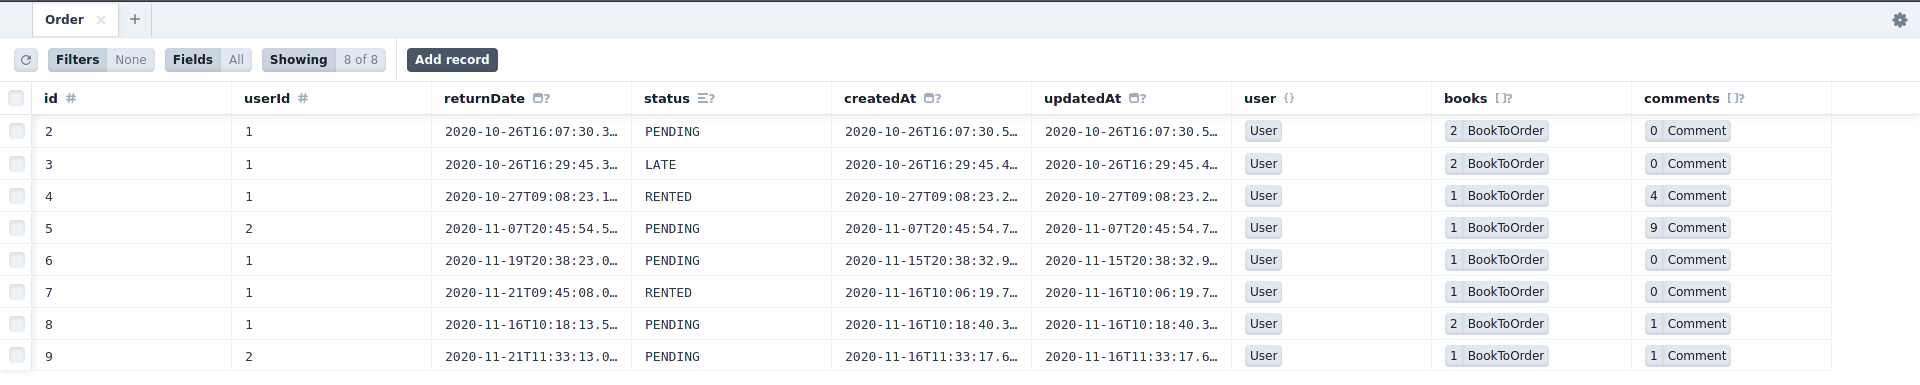
\includegraphics[width=150mm, keepaspectratio]{figures/prisma-studio.png}
\caption{A Prisma Stuio felülete}
\label{fig:DBSchema}
\end{figure}
